\documentclass{article}
\usepackage{graphicx} 
\usepackage{hyperref}

\title{Advanced programming for HPC - Labwork 4}
\author{Son Dang Thai}
\date{October 2025}

\begin{document}

\maketitle

\section{Improvement}
This labwork was carried out on a 512x512 image

\begin{figure}[!htb]
    \begin{minipage}{0.48\textwidth}
        \centering
        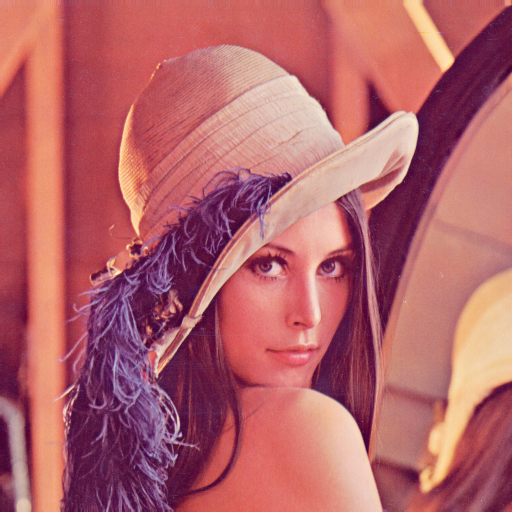
\includegraphics[width=.7\linewidth]{lenna.png}
        \caption{Experiment photo}
        \label{fig:rgb}
    \end{minipage}\hfill
    \begin{minipage}{0.48\textwidth}
        \centering
        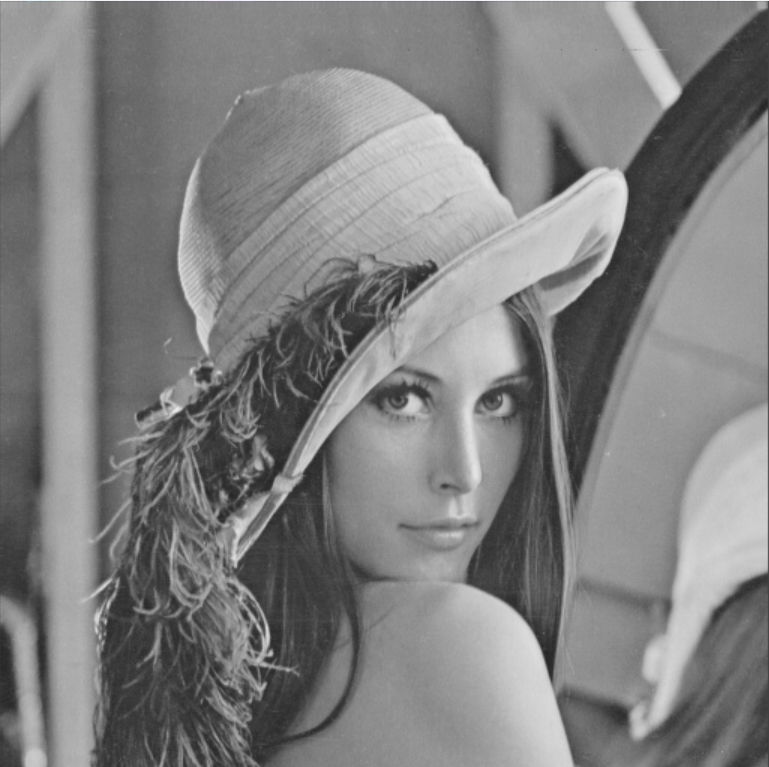
\includegraphics[width=.7\linewidth]{lenna_grayscale.png}
        \caption{Grayscale result}
        \label{fig:grayscale}
    \end{minipage}\hfill
\end{figure}

Instead of flattening an RGB image into 1 dimension, the grayscale converting function here kept its original 2D structure.

\begin{itemize}
  \item For CPU use: there were 2 nested for loops to iterate over all width and height of the image. The conversion algorithm was kept the same: gray\_value = (red + green + blue) / 3
  \item For GPU use: due to working with a 2D dimension, each thread's position had to be defined by a coordination set (x, y) defined by local\_threadId + blockId * blockDimension. The conversion algorithm was kept the same. Besides, there was a major improvement on recording the response time: the GPU function was run once to remove the odd before it actually started to record the time.
\end{itemize}

\section{Response time}
\subsection{Grayscale using CPU}
Compared to the time recorded using labwork 3 (0.27 seconds), using 2 nested for loops took around 0.3 seconds, which was a bit longer.

\subsection{Grayscale using GPU}

\begin{figure}[!htb]
    \begin{minipage}{0.48\textwidth}
        \centering
        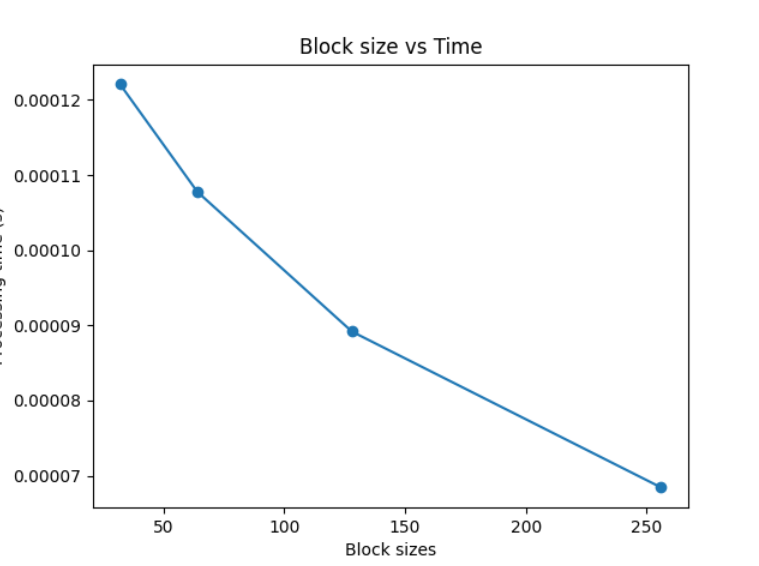
\includegraphics[width=.7\linewidth]{GPU response time 1D.png}
        \caption{Response time on 1D}
        \label{fig:1D response time}
    \end{minipage}\hfill
    \begin{minipage}{0.48\textwidth}
        \centering
        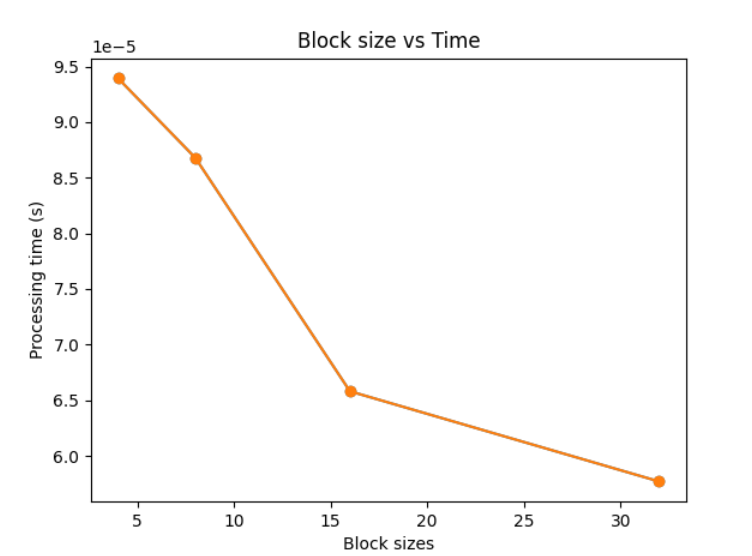
\includegraphics[width=.7\linewidth]{GPU response time 2D.png}
        \caption{Response time on 2D}
        \label{fig:2D response time}
    \end{minipage}\hfill
\end{figure}

From experiments using labwork 3: block sizes of [32, 64, 128, 256] gave response time was of [0.0001220703125, 0.00010776519775390625, 8.916854858398438e-05, 6.842613220214844e-05] seconds respectively.

When working with 2D grid of block sizes [(4, 4), (8, 8), (16, 16), (32, 32)], the resposne time was recorded at [9.393692016601562e-05, 8.678436279296875e-05, 6.580352783203125e-05, 5.7697296142578125e-05] seconds, which implies the larger the block size, the shorter the response time.

This shows that working with 2D RGB images using GPU is a lot faster than working with converted 1D images.

\section{Exercises}
\subsection{Exercise 1}
The best configuration for thread blocks to implement grayscaling is 16x16.

\begin{itemize}
  \item There are 16 x 16 = 256 threads/block
  \item This is valid for 32 threads/warp and maximum of 512 threads/block
  \item There are 1024 / 256 = 4 blocks/SM which is valid for maximum of 8 blocks/SM
  \item In total, there are 256 x 4 = 1024 threads/SM which shows 100\% occupancy
\end{itemize}

The 8x8 one only has 50\% occupancy and the 32x32 one has more than 512 threads/block

\subsection{Exercise 2}
The block configuration resulting in the most number of threads in the SM is 512 threads/block

\begin{itemize}
  \item There are 1536 / 512 = 3 blocks in total which satisfies maximum of 4 blocks
  \item Putting 3 blocks of 512 threads/block, we get total 1536 threads in the SM (maximum number)
\end{itemize}

For 128 threads/block: there are only 512 threads with 4 blocks

For 256 threads/block: there are only 1024 threads with 4 blocks

For 1024 threads/block: there are only 1024 threads with 1 blocks

\subsection{Exercise 3}
\begin{itemize}
  \item With 2000 threads there are 2000 / 512 = 3.90625 = 4 blocks
  \item So in total there are 512 x 4 = 2048 threads in the grid
\end{itemize}

\end{document}
